\section{Introduction}
Quantum computation, a paradigm of computing that is completely different from 
classical methods, shows potential to solving classically intractable computational 
problems in areas such as quantum chemistry, cryptography, machine learning, 
and others. The ideal quantum computer should be composed of a top-down system stack, 
which is roughly divided into the top layer of quantum language and algorithm, 
the middle layer of control hardware and bottom layer of quantum processor. 
Recently, google used a programmable superconducting processor to solve a 
specific computational task, which can be regarded as an experimental 
realization of quantum supremacy. With the rapid progress of quantum processor, 
finding out a general architectural solution of control hardware for bridging 
the gap between quantum language and quantum processor is becoming increasingly urgent.

Since dedicated electronic devices which are used to apply well-defined electrical signals 
on quantum processor introduce high resource consumption, long configuration times, 
and control complexity, which seriously limited the scalability, Fu. etc propose a prototype of 
control microarchitecture (QuMA V2) based on circuit model that translates a set of instructions into the 
interface required by a quantum processor. QuMA V2 can relize quantum circuit with little memory overhead, 
as well as support feedback control, which is important for some quantum algorithms,such as ....(其他组的工作)

However, the hardware constraints of quantum processors pose new challenges to the design of 
quantum computing architecture. On the one hand, the waveform parameters of quantum gates fluctuates due to the 
influence of environmental noise, therefore, supporting waveform calibration is necessary for the full stack 
quantum computing architecture to improve the accuracy of the results of quantum circuit. The execution of quantum 
application should include two steps:  waveform calibration and quantum circuit execution. 
In particular, for some quantum applications that need to determine the rotation angle of quantum gates 
used in the next iterative circuit based on the measurement results, such as QAOA, the quantum computing 
architecture also needs to support new waveform generation. For it is impossible to pre-calibrate and store 
all possible waveforms into the waveform library since the rotation angle is continuous and unpredictable 
for each iteration. Figure~\ref{img} shows the quantum program execution flow. On the other hand, waveform compensation 
method is used to reduce the negative effects of crosstalk of DC pulses, reducing the fidelity of quantum gates. 
Using compensating method means that pulses on qubit become contextual --- dependent on what is being played 
simultaneously on other qubits. 

\begin{figure}[ht]
  \centering
  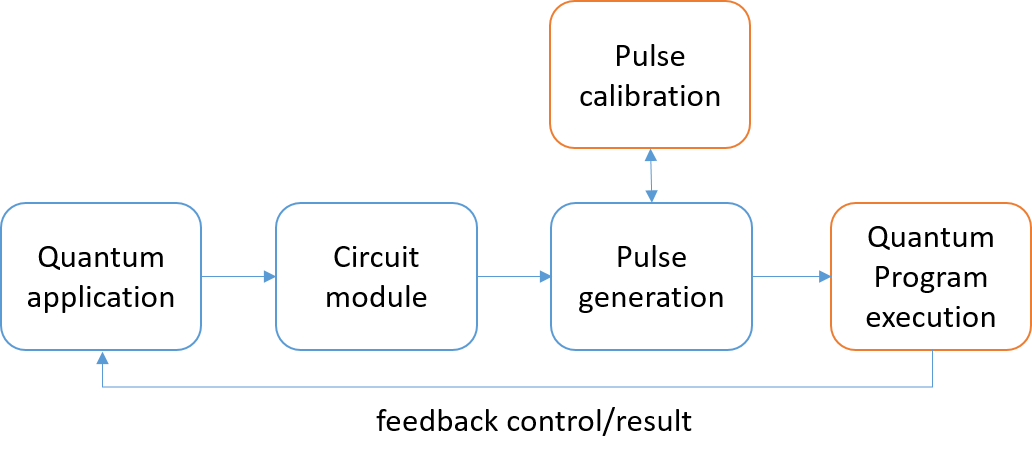
\includegraphics[width=\linewidth]{figure/1}
  \caption{The execution flow of quantum application}
  \label{img}
\end{figure}

The control microarchitecture based on the gate model, that at each timestamp only one pulse for corresponding 
quantum gate act only on the target qubit, is hard to support above two situation. To this end, we propose a quantum control 
micro-architecture based on electrode event, namely ebQuMA. There are three core concepts:
\begin{itemize}
  \item Electrode event based quantum operation unit: The basic unit of quantum operation is the electrode event, which is an abstraction of the waveform applied on one electrode, 
  including waveforms of one quantum gate or a combination of quantum gates over a period of time, 
  calibration experiment and optimized waveform for partial quantum circuit. 
  Each qubit requires multiple types of electrode events that can be applied on the qubit simultaneously, depend on the control architecture of the quantum processor. 
  This solution allows the microarchitecture to control the quantum processor at the electrode level, providing the foundation for supporting calibration experiments and waveform compensation. 
  \item Hybrid event description scheme: Quantum operation instructions are divided into global event 
  operations and local event operations. Local event operations need to specify qubits that execute the event, while global 
  event operations execute the event on all qubits. It provides a simpler description scheme for quantum operations that 
  require compensation, compared with specifying different events for each qubit in turn. In addition, this scheme can 
  also greatly reduce the instruction overhead for the descriptions of the quantum circuit with high gate diversity.
  \item Multi-level compilation scheme: The compilation of quantum application is divided into three steps: compiling 
  the quantum program into a quantum assembly program based on electrode events, generating waveform files for each event, 
  and mapping encoding of each event and the storage address of corresponding waveform. It reduces the task of the 
  microarchitecture at runtime by implementing waveform compensation and waveform generation of high gate diversity 
  circuits at compiling time, thereby improving the issue rate problem.
\end{itemize}

The paper is structured as follows. Section 2 briefly introduces the basics of the control method of superconducting qubits. 
Section 3 presents related previous work. We state the challenges of microarchitecture design 
and our solution with three proposed schemes, respectively in Sections 4 and 5. 
Section 6 discusses the implementation of ebQASM. 
The advantages and resource costs are evaluated in Section 7. 
Section 8 concludes.